\documentclass[twocolumn, 10.5pt]{article}
\usepackage{verbatim}
\usepackage{amsfonts}
\usepackage{geometry}
\usepackage{amsmath}
\usepackage{amsthm}
\usepackage{amssymb}
\usepackage{listings}
\usepackage{graphicx}
\usepackage{clrscode3e}
\usepackage{txfonts}
\usepackage{fontspec}
\usepackage{ctex}
\usepackage{float}
\setmainfont{Times New Roman}
\geometry{top=2.5cm,bottom=2.5cm,left=2.5cm,right=2.5cm}
\setlength\parindent{0em}
\begin{document}
	\title{Problem Solving Homework (Week 4)}\author{161180162 Xu Zhiming}\maketitle
	\section*{JH Chapter 3}
	\subsection*{3.4.2.1}
		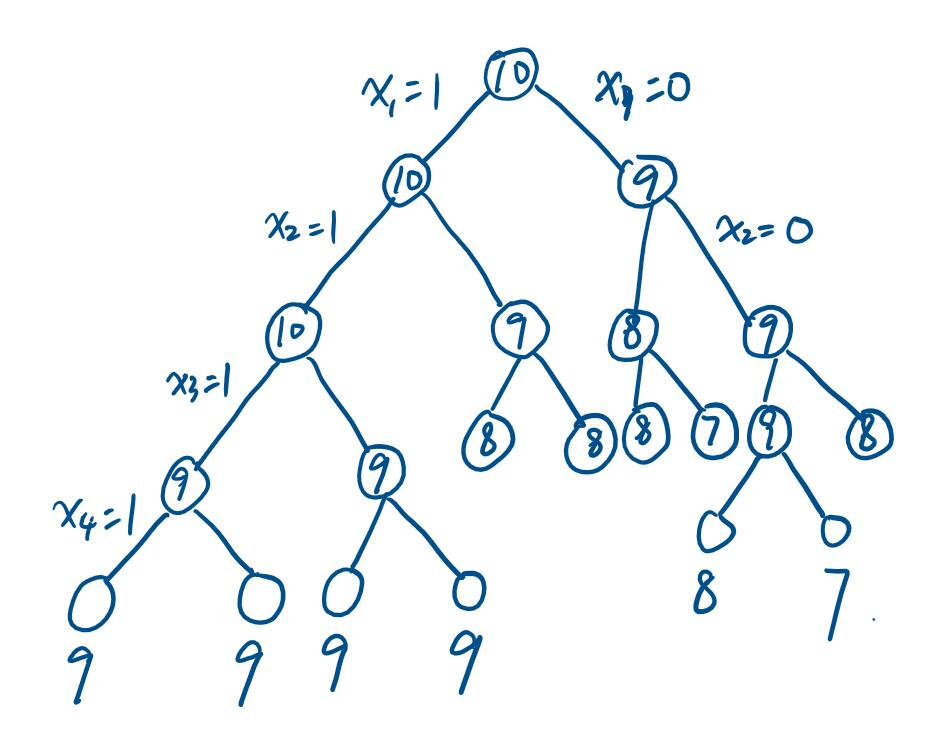
\includegraphics[scale=0.32]{ex4-1.jpg}
	\begin{figure}[H]
		\centering
		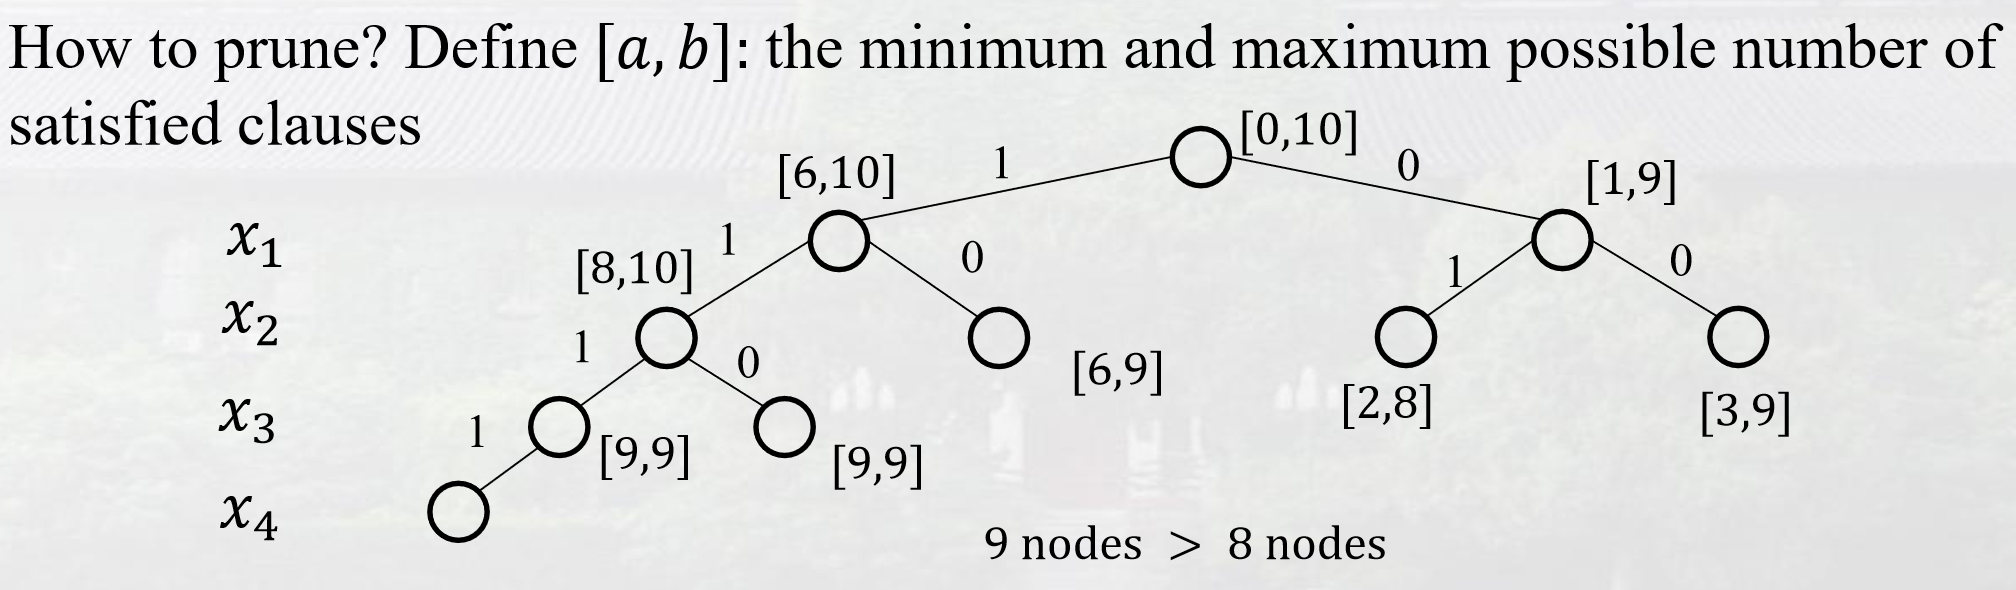
\includegraphics[width=1\linewidth]{hw4-2.png}
		\caption{\textbf{REVISE}}
	\end{figure}
	\subsection*{3.4.2.2}
	This is right DFS's search tree:\\
	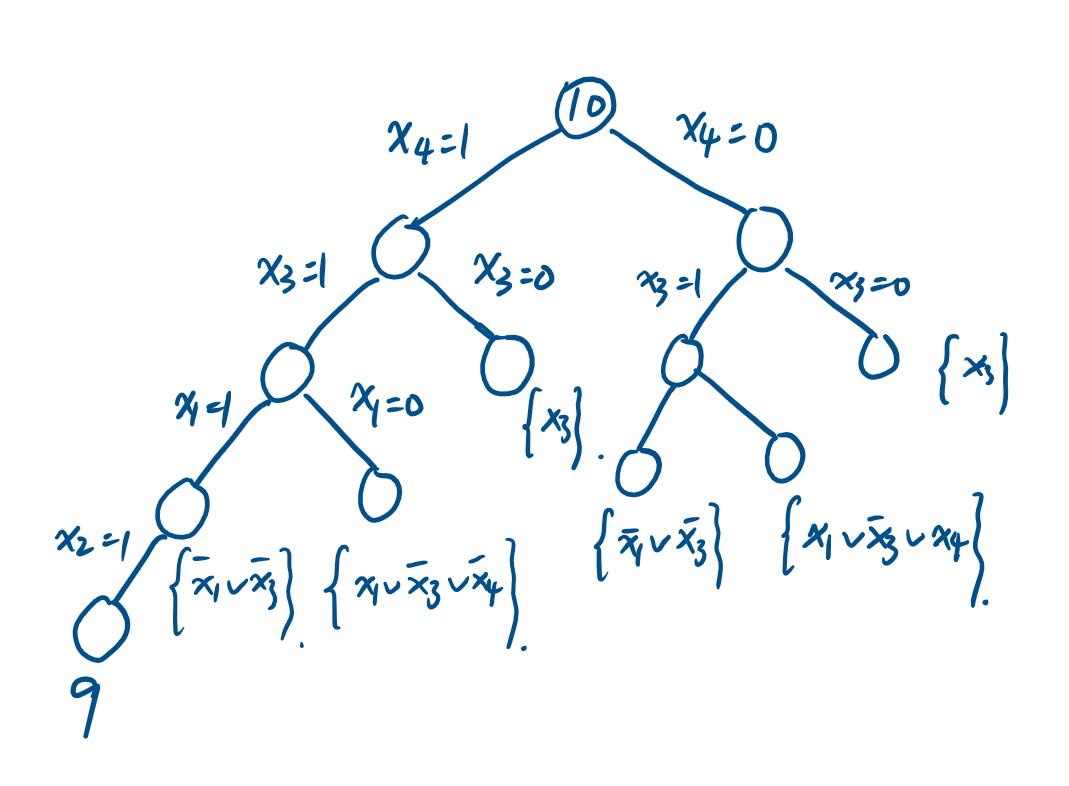
\includegraphics[scale=0.31]{ex4-2.jpg}
	This is left DFS's search tree:\\
		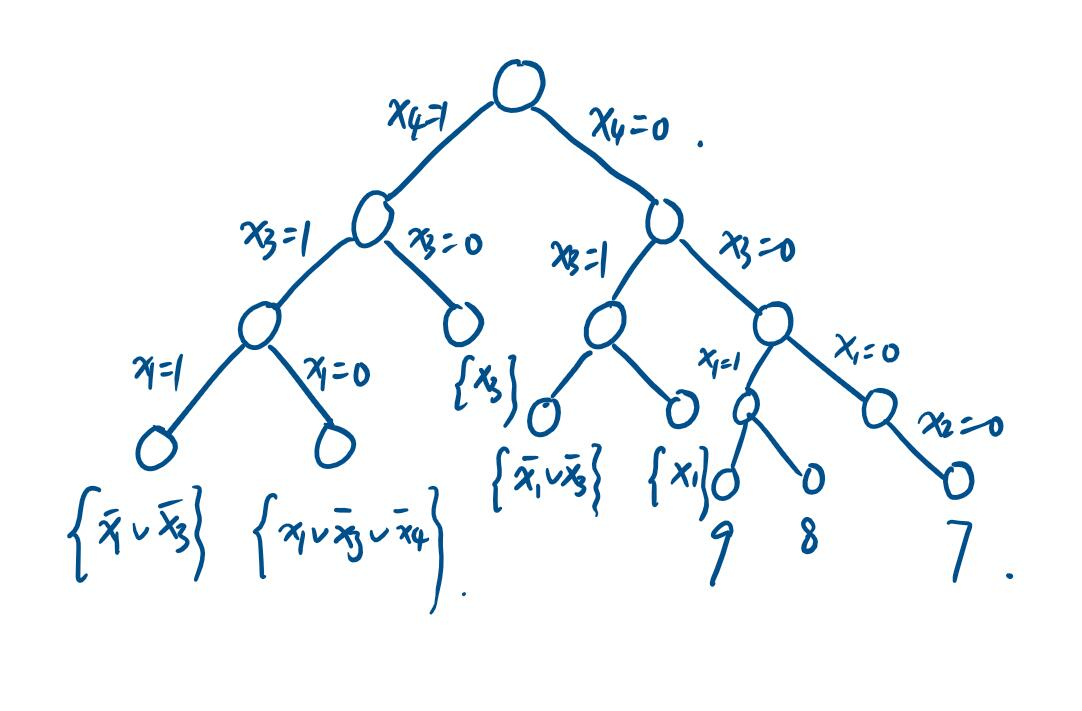
\includegraphics[scale=0.32]{ex4-3.jpg}
	\subsection*{Knapsack}
	Sort all items by its cost, in ascending order. The enumerate all possibilities. A favorable instance can be \{W,C,b\}=\{2,3,4,1,2,3,4\}, and an unfavorable instance can be \{W,C,b\}=\{4,3,2,1,2,3,4\}. 
\end{document}